\chapter{Basic engineering}\label{chap:Basic engineering}

\section{Checkliste}\label{sec:Checkliste}

Siehe Checkliste unter <Projektordner> 03.Basic Engineering, Safety

\begin{figure}[!ht]
    \centering
    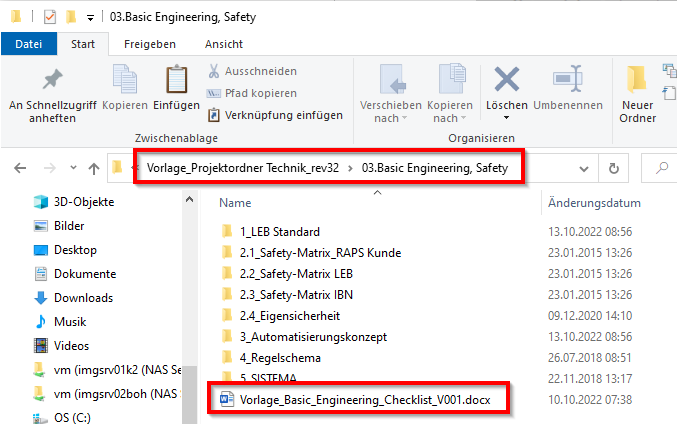
\includegraphics[width = 0.8 \textwidth]{Basic Engineering Checklist Ablageort.png}
    \caption{Basic Engineering Checklist Ablageort}
    \label{fig:Basic Engineering Checklist Ablageort}
\end{figure} 

\noindent \textbf{Diese Liste ist zu Beginn eines jeden Projektes durchzuarbeiten und auszufüllen!}

\clearpage
\section{Beispiele, warum Basic Engineering wichtig ist}\label{sec:Beispiele, warum Basic Engineering wichtig ist}

\subsection{1-kanaliger induktiver Sensor PLd -> besondere Beschaltung}\label[]{subsec:1-kanaliger induktiver Sensor PLd -> besondere Beschaltung}

Sensor: SICK IN40-D0303K

\begin{figure}[!ht]
    \centering
    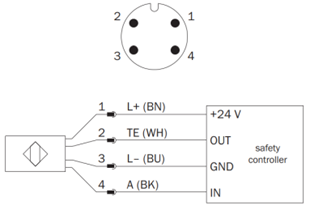
\includegraphics[width = 0.5 \textwidth]{SICK IN40 - D030K - Schaltbild.png}
    \caption{SICK IN40 - D030K - Schaltbild}
    \label{fig:SICK IN40 - D030K - Schaltbild}
\end{figure} 

\begin{figure}[!ht]
    \centering
    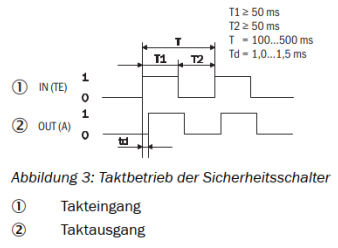
\includegraphics[width = 0.5 \textwidth]{SICK IN40-D0303K - Signalverhalten.png}
    \caption{SICK IN40-D0303K - Signalverhalten}
    \label{fig:SICK IN40-D0303K - Signalverhalten}
\end{figure}

\clearpage

\noindent Schaltungsbeispiel:

\begin{figure}[!ht]
    \centering
    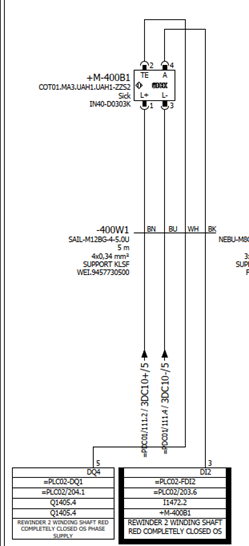
\includegraphics[width = 0.5 \textwidth]{Induktiver Sensor 1-kanalig PLd Schaltungsbeispiel.png}
    \caption{Induktiver Sensor 1-kanalig PLd Schaltungsbeispiel}
    \label{fig:Induktiver Sensor 1-kanalig PLd Schaltungsbeispiel}
\end{figure}

\noindent Um in 1-kanaliger Ausführung PLd zu erreichen, muss der Sensor selbst überwachen, dass eingangsseitig kein (Anschluss TE) kein Kurzschluss vorliegt. Daher ist auf dem Kanal ein gepulstes Signal vorzusehen, ansonsten geht der Sensor von einem Fehler aus und schaltet auch bei Betätigung nicht mehr.
Softwareseitig bietet Siemens dazu eine Lösung, die unter dem folgenden Link zu finden ist:

\noindent \url{https://support.industry.siemens.com/cs/document/109818998/sicheres-erfassen-mit-induktiver-taktender-sensorik-bis-sil-3-pl-d?dti=0&lc=de-DE} % \- for manual line break in url if necessary

\noindent Beitrags-ID SIOS: 109818998

\cite[\textbf{TODO!}]{todo}
